\documentclass{article}
\usepackage{tikz-cd}
\usepackage{amsmath}
\usepackage{mathrsfs}

\usetikzlibrary{positioning,shapes.geometric,fit}

\title{Counterexamples in Mathematical Relations}
\author{}
\date{}

\begin{document}

\maketitle

\section{Introduction}
This document contains diagrams of counterexamples commonly encountered when exploring the properties of mathematical relations.

\section{Counterexamples}

\subsection{Counterexample 1}
\begin{center}

    \begin{tikzcd}[node distance=2cm, auto]
        % Nodes
        \node (a) {a};
        \node (b) [right of=a, xshift=1cm] {b};
        \node (c) [right of=b, xshift=1cm] {c};
        \node (d) [right of=c, xshift=1cm] {d};

        % Arrows
        \draw[->] (b) to [bend left] (c);
        \draw[->] (c) to [bend left] (b);
        \draw[->] (b) -- (a);
        \draw[->] (c) -- (d);
    \end{tikzcd}

\end{center}
Counterexample to:
\begin{itemize}
    \item WCR $\to$ CR
    \item WCR and WN $\to$ CR
    \item WCR and WN $\to$ SN
    \item \mbox{WCR R $\to$ $\forall$ a b $\to$ is R -NF b $\to$ (R *) a b $\to$ $\forall$ c $\to$ (R *) a c $\to$ (R *) c b}
    \item IOW, WCR $\to$ WNFP
\end{itemize}

\subsection{Counterexample 2}
\begin{center}
    \begin{tikzcd}
        % Nodes
        \node (x) {x};
        \node (n) [below left of=x, xshift=-1cm, yshift=-1cm] {n \in NF};
        \node (y) [below right of=x, xshift=1cm, yshift=-1cm] {y};
        \node (z) [below of=y, yshift=-1cm] {z};

        % Arrows
        \draw[->>] (x) -- (n);
        \draw[->>] (x) -- (y);
        \draw[->] (y) to [bend left] (z);
        \draw[->] (z) to [bend left] (y);
    \end{tikzcd}
\end{center}

Counterexample to:
\begin{itemize}
    \item WN$\downarrow\subseteq$WN :  $\forall$ x $\to$ is R-WN x $\to$ $\forall$ y $\to$ (R *) x y $\to$ is R-WN y
    \item WN$\downarrow$UN$\rightarrow\subseteq$WN :

    UN$\rightarrow\,$R $\to \forall$ x $\to$ is R-WN x $\to$ $\forall$ y $\to$ (R *) x y $\to$ is R-WN y

    \textcolor{red}{SA: The above is a bit messy, can we make it cleaner?}
    \item $\forall$ (R : $\mathscr{R}$ A) $\to$ $\forall$ is R -WN x $\to$ is R -UN x $\to$ is R -CR x

\end{itemize}

\subsection{Counterexample 3}
\begin{center}
  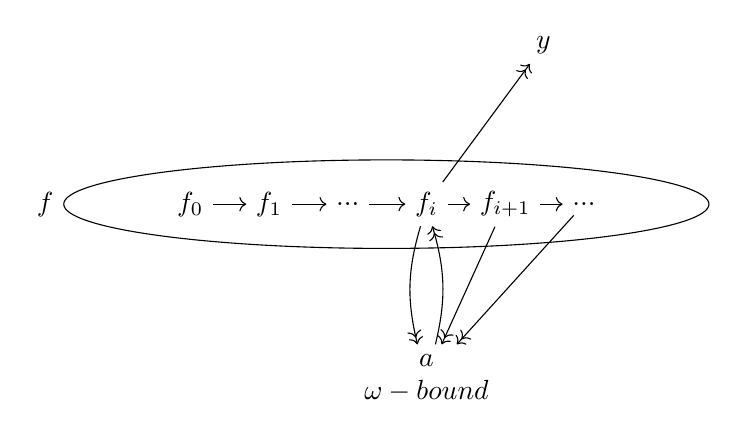
\begin{tikzpicture}
      % Define the nodes inside the region f
      \node (f0) at (0, 0) {$f_0$};
      \node (f1) at (1, 0) {$f_1$};
      \node (fi) at (3, 0) {$f_i$};
      \node (fi+1) at (4, 0) {$f_{i+1}$};
      \node (dots) at (2, 0) {$...$};
      \node (dots2) at (5, 0) {$...$};

      % Draw the arrows between the nodes inside the region f
      \draw[->] (f0) -- (f1);
      \draw[->] (f1) -- (dots);
      \draw[->] (dots) -- (fi);
      \draw[->] (fi) -- (fi+1);
      \draw[->] (fi+1) -- (dots2);

      % Define the region f
      \node[draw, ellipse, fit=(f0) (dots2), label=left:$f$] {};

      % Define the nodes outside the region f
      \node (a) [below=of fi, yshift=-.5cm] {\parbox{2cm}{\centering $a$ \\ $\omega-bound$}};
      \node (y) [above right=of fi, yshift=.5cm] {$y$};

          % Draw the arrows between the nodes inside and outside the region f
          \draw[->>] (fi) to [bend right=15] (a);
          \draw[->>] (a) to [bend right=15] (fi);
          \draw[->>] (fi+1) -- (a);
          \draw[->>] (dots2) -- (a);
          \draw[->>] (fi) -- (y);
      \end{tikzpicture}
    \end{center}
    Counterexample to:
    \begin{itemize}
      \item ***** DOES NOT WORK ******
      \item RP-$\to$RP 
      \item RP-$\land$WCR$\to$RP \textcolor{red}{NO< NEEDS A NEW CE}
\end{itemize}

\subsection{Other questions}
\begin{enumerate}
  \item If WCR holds, is WN$\downarrow\subseteq$WN ?
  \item Same question for next bullet in 2.2
  \item Same for bullet 3 in 2.2 (but pointwise!)
  \item Do RP- $\land$ WCR imply RP?
\end{enumerate}
\subsection{ARS in Agda}
Important counterexamples:
\begin{enumerate}
  \item $a,b,c,d$ with sinks $a$ and $d$ and a 2-cycle between $b$ and $c$.
  Counterexample to:
  \begin{itemize}
      \item WCR and WN implies CR.
  \end{itemize}
  \item Loop $a \to a$.
  Counterexample to:
  \begin{itemize}
    \item $\omega$-bounded and RP implies SN
    \item $\omega$-bounded and RP implies WN
  \end{itemize}
  \item Infinite sequence $a_0 \to a_1 \to \cdots$. Falsifies:
  \begin{itemize}
    \item $WN$
    \item $\omega$-bounded
    \item RP $\to$ $\omega$-bounded
    \item $WCR \to WN$
    \item $CR \to WN$
    \item $CR, CP \to WN$
    \item $CR, CP \to \omega$-bounded
  \end{itemize}
  \item Infinite sequence $a_0 \to a_1 \to \cdots$ with a colimit $a_\infty$,
  with each $a_n \to a_\infty$ and $a_\infty$ a normal form.

  Counterexample to:
  \begin{itemize}
    \item WN $\to$ SN
    \item WN, CR $\to$ SN
    \item WN, CR, $\omega$-bounded $\to$ SN
  \end{itemize}

  \item Infinite sequence $a_0 \to a_1 \to \cdots$, together with links
  $a_n \to a_0$, for each $n$.
  \item The combination of the last two.
  Counterexample to
  \begin{itemize}
    \item RP
  \end{itemize}
  \item An ``infinite haircomb''. Infinite sequence $a_0 \to a_1 \to \cdots$, together with
  a disjoint, discrete set $b_0, b_1, \dots$, and links $a_n \to b_n$.
  Counterexample to:
  \begin{itemize}
    \item $WN\to WCR$
    \item $WN\to \omega-bounded$
    \item $WN \to SN$
    \item $WN,RP \to SN$
  \end{itemize}
  \item A variation of the above with backlinks $a_n \to a_0$ for all $n$.
\end{enumerate}


\end{document}
